\chapter{Giới thiệu đề tài}
\pagestyle{fancy}
Từ lúc bắt đầu có khái niệm IoT cho đến nay, đã có rất nhiều ứng dụng trong những lĩnh vực khác nhau, mang lại hiệu quả và độ chính xác cao hơn hẳn so với sức người, giảm chi phí cho sản xuất, bảo vệ môi trường,... Do đó, IoT được dự báo là công nghệ của tương lai, đóng vai trò quan trọng trong \lq\lq{}Cách mạng công nghiệp 4.0\rq\rq{}.\\

Hình dưới đây mô tả một hệ thống IoT tiêu chuẩn: các thiết bị và cảm biến trong nhóm Things sẽ kết nối, giao tiếp với nhau thông qua một mạng nội bộ, một số ứng dụng chỉ cần nhóm này là đủ nếu không có nhu cầu trao đổi dữ liệu với cloud. Gateway sẽ đảm nhiệm vai trò kết nối giữa hai loại mạng khác nhau, chẳng hạn như mạng nội bộ với cloud, mạng WiFi với ZigBee hay như trong đề tài này là mạng Bluetooth Mesh với GPRS. Sau cùng là cloud với vai trò lưu trữ dữ liệu cũng như phân tích nó, cloud còn đảm nhiệm giao tiếp với một số thiết bị có giao diện người dùng như máy tính, điện thoại,...

    \begin{figure}[h!]
    	\begin{center}
    		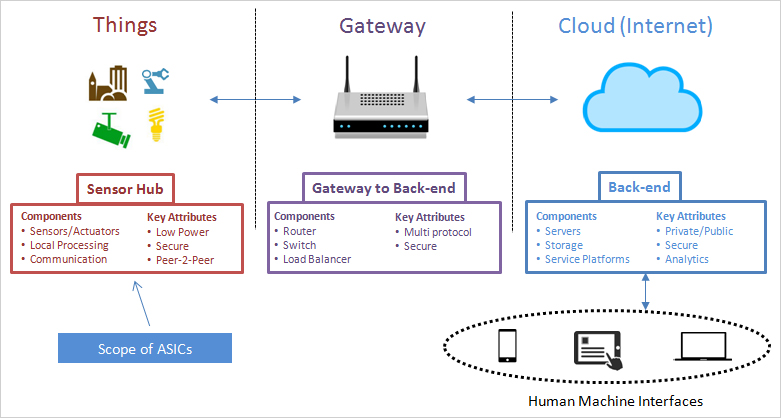
\includegraphics[scale=0.5]{images/internet-of-things-bone.jpg}
    		\caption{Một hệ thống IoT tiêu chuẩn}
    	\end{center}
    \end{figure}

Nhóm Things có thể bao gồm rất nhiều thiết bị, chẳng hạn như một hội trường cỡ vừa đã có hàng trăm bóng đèn, hàng trăm cái ghế. Do đó việc sử dụng kiểu kết nối hình sao, vòng, P2P hay cây đều có những bất lợi cũng như khó mở rộng, kết nối mesh dễ dàng đánh bại những kiểu kết nối khác trong cuộc đua này.\\

Cho đến nay đã có rất nhiều giải pháp mạng mesh không dây (wireless) sử dụng nhiều loại công nghệ khác nhau. Mục tiêu ban đầu của những giải pháp này là ứng dụng trong quân sự, sau đó là công nghiệp và cuối cùng là nhà thông minh. Lý do chính dẫn đến thất bại của WiFi và ZigBee trong việc hiện thực mạng mesh chính là thiếu khả năng liên kết giữa các nhà sản xuất, Bluetooth Mesh sẽ thay đổi điều đó\cite{meshadvan}.\\

Nhằm tìm hiểu tiềm năng trong tương lai của Bluetooth Mesh, nhóm đã thực hiện đề tài này và tổng hợp những điểm quan trọng của giao thức này trong báo cáo, làm cơ sở tham khảo cho những ai quan tâm và có ý định phát triển ứng dụng trên nền Bluetooth Mesh.\\

Báo cáo sẽ được trình bày theo thứ tự như sau:
    \begin{itemize}
        \item Chương đầu tiên sẽ giới thiệu sơ lược về đề tài và giao thức Bluetooth Mesh, liệt kê những nhiệm vụ cần đạt cũng như sơ đồ khối và cách thức hoạt động của ứng dụng thử nghiệm.
        \item Chương tiếp theo sẽ tập trung vào những gì nhóm nghiên cứu được về giao thức Bluetooth Mesh, điểm qua lịch sử, kiến trúc, nguyên lý hoạt động và cách thức quản lý các phần tử trong mạng.
        \item Chương 3 là danh sách những công cụ cả về phần cứng và phần mềm mà nhóm dùng để hiện thực ứng dụng thử nghiệm, có bao gồm mô hình thiết kế của ứng dụng.
        \item Chương 4 ghi lại quá trình hiện thực ứng dụng dựa trên công cụ của nhà sản xuất và tùy chỉnh một số mã nguồn mẫu, hiện thực thư viện giao tiếp với module GSM.
        \item Chương 5 là các kịch bản nhóm dựng lên để thử nghiệm ứng dụng, bao gồm thử nghiệm khoảng cách tối đa giữa 2 thiết bị trong mạng, giao tiếp trong mạng và hoạt động của node gateway.
        \item Chương 6 là chương kết luận, bao gồm việc đánh giá và đưa ra gợi ý cho những ứng dụng trong thực tế.
        \item Cuối cùng là tài liệu tham khảo và một số phụ lục: các model chuẩn, flowchart quá trình remote provisioning, hướng dẫn sơ lược cách sử dụng các chương trình nhóm dùng để hiện thực ứng dụng.
    \end{itemize}

    \section{Nhiệm vụ cần đạt}
    \begin{itemize}
        \item Tìm hiểu lý thuyết về Bluetooth Mesh, nguyên lý hoạt động, ưu nhược điểm,... Mục tiêu này đã hoàn thành bước đầu trong giai đoạn Đề lương luận văn. Giai đoạn luận văn sẽ nghiên cứu sâu hơn và cụ thể hơn các lý thuyết đã được trình bày ở giai đoạn Đề cương.
        \item Sử dụng các công cụ hiện có, hiện thực ứng dụng có khả năng giao tiếp giữa các thiết bị cuối - đảm nhiệm nhiệm vụ thu nhập dữ liệu và điều khiển thiết bị - và thiết bị gateway - đảm nhiệm việc giao tiếp với cloud.
        \item Đề ra các phương án áp dụng Bluetooh Mesh vào các ứng dụng thực tế, cũng như các hướng phát triển trong tương lai.
        \item Xây dựng kịch bản để thử nghiệm, chứng minh ưu điểm của Bluetooth Mesh so với các chuẩn giao tiếp khác.
    \end{itemize}
    \newpage
    \section{Sơ đồ khối}

    \begin{figure}[h!]
    	\begin{center}
    		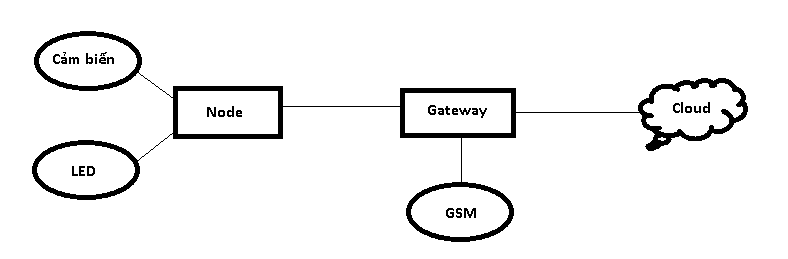
\includegraphics[scale=0.8]{images/block-diagram.png}
    		\caption{Sơ đồ khối của ứng dụng}
    	\end{center}
    \end{figure}

    \section{Hoạt động}
        \begin{itemize}
            \item Trước tiên cần tiến hành bước khởi tạo: cho phép các node cảm biến tham gia vào mạng.
            \item Ấn nút trên node gateway để kích hoạt/tắt chức năng giám sát của hệ thống. Khi trong chế độ giám sát, sau mỗi chu kỳ nhất định, node gateway sẽ gửi yêu cầu lần lượt tới toàn bộ các node cảm biến có trong mạng - quá trình này cũng cho phép kiểm tra sự tồn tại của các node trong mạng - sau đó gửi toàn bộ dữ liệu lên server. Chức năng này thể hiện hướng dữ liệu từ node cảm biến đến node gateway.
            \item Ấn một nút khác cũng trên node gateway để điều khiển LED trên tất cả các node cảm biến, chức năng này giúp cho việc kiểm thử dễ dàng hơn. Chức năng này thể hiện hướng dữ liệu từ node gateway đến node cảm biến.
        \end{itemize}

